\documentclass[12pt,a4paper]{article}
\usepackage[utf8]{inputenc}
\usepackage{graphicx}
\usepackage{cancel}
\usepackage[margin=1in]{geometry}
\title{Python core}
\author{Anivarth Peesapati}
\begin{document}
\begin{flushleft}
.
\end{flushleft}
\begin{flushright}
.
\end{flushright}
\vspace{7cm}
\begin{center}
\begin{Huge}
\textbf{Python Core}
\end{Huge}
\\

\begin{huge}
Python - I
\end{huge}
\\
\begin{normalsize}
Python 2.7 Docs
\end{normalsize}
\end{center}
\begin{flushright}
\begin{LARGE}
Anivarth Peesapati
\end{LARGE}

\begin{large}
January 2016
\end{large}

\begin{normalsize}
ver. 1.0
\end{normalsize}
\end{flushright}
\clearpage
\tableofcontents\clearpage
\section{Introduction}
When we pass the arguments to the interpreter then the values are stored in the \texttt{argv} variable in the  \texttt{sys} module. It is better to add \texttt{\# -*- coding: encoding -*-} at the begining of every script so that the interpreter understands the unicode that in which the python code is being written. For UTF-8 we add \texttt{\# -*- coding: UTF-8 -*-}
\section{Comments}

Comments in python start with \texttt{\#}. It can be included at any place. But they cannot be used inside a string. 

\texttt{\\
\# This is a comment\\
name = "Anivarth"\\
string = "\#This is not a comment, but a string."
}

\section{Mathematics with Python}

All the arithmetic operations can be done with python. Addition(\texttt{+}), subtraction(\texttt{-}), multiplication(\texttt{*}), division(\texttt{/}).

\texttt{\\
>>> 2+3\\
5\\
>>> 5*6\\
30
}
\linebreak
\linebreak
Power of a number can be calculated using \texttt{**} and remainder using \texttt{\%}.

\texttt{\\
>>> 2**2\\
4\\
>>> 5**2\\
25\\
>>> 5\%2\\
1}
\linebreak
\linebreak
Operator precedence in python is \texttt{(), **, *, /, \%, //, +, -}.\footnote{Since ** has higher precedence than -, -3**2 will give result as -(3**2), but to get exact value we will have to use (-3)**2}
\subsection{Division with python}
Usually if we divide two integers python does a floor division and returns the output. Integers in the sense the numbers without any point after it. But if we want to get the real value of the division we will have to type any one of the number(either numerator or denominator) as a float number.

\texttt{\\
\\
>>> 5/7\\
0\\
>>> 5.0/7\\
0.7142857142857143\\
>>> 3.5/6.8\\
0.5147058823529412
}
\linebreak
\linebreak
If we want to strictly perform floor division then we can use \texttt{//}

\texttt{\\
>>> 3.5//6.8\\
0
}


\section{Variables in Python}
\texttt{'='} is used to assign variables in python.Last printed expression is given the value \texttt{\_}. It should be remembered that the variable \texttt{\_} can only be used as read only and cannot be assigned any values. We can also create variables with complex numbers. We can also perform calculations with complex numbers. If we try to use any variable without defining it then it will give a traceback error. 


\texttt{
\\
>>> name = "Anivarth"\\
>>> \# Using \_ now will give a variable undefined error.\\
>>> 3+6j\\
>>> \_\\
>>> 3+6j\\
>>> round(5.985,2)\\
5.99\\
>>> anivarth\\
Traceback error}



\section{Strings}
Stings in python are created using '....' or "...." for one line stings. \texttt{'$\setminus$'} is used for escape sequences. To create multiple line strings we use """....""" or '''.....'''. To remove line break we use '$\setminus$'.

\texttt{\\
>>> 'spam eggs'\\
'spam eggs'\\
>>> '"Isn$\setminus$'t," she said'\\
'"Isn$\setminus$'t," she said'\\
>>> print """$\setminus$\\
Usage: thingy \\
This is a multiline string."""}
\subsection{Raw strings in python}
To create raw strings (i.e. stings in which what ever is entered is returned) we use '\texttt{r}' in front of the string and the raw text is returned.
\texttt{\\
>>> print r"C:$\setminus$some$\setminus$name"\\
C:$\setminus$some$\setminus$name\\ 
>>> print "C:$\setminus$some$\setminus$name"\\
C:$\setminus$some\\
ame\\
>>> \#This is because of the $\setminus$n in code \\
}

\subsection{String concatenation and multiplication}
In python two strings are concatenated using '\texttt{+}' and multiplied using '\texttt{*}'. But if we have two strings just by placing them side by side we can concatenate them. Concatenating just by placing them side by side is not possible when variables are used. To concatenate multiple sentences place them in parenthesis and they are concatenated. 

\texttt{\\
>>> 3*'un'+'ium'\\
'unununium'\\
>>> 'Py' 'thon'\\
'Python'\\
>>> \# The following will not work\\
>>> prefix = 'Py'\\
>>> prefix 'thon'\\
SyntaxError:\\
>>> prefix+'thon'\\
'Python'\\
>>> \# More than one sentences.\\
>>> text = ('Put several strings within parenthesis'\\
 'to have them joined together.')\\
>>> text\\
'Put several strings within parenthesis to have them joined together.'\\
}
\subsection{String Indexing and slicing}
Strings can be indexed(subscripted), with the first character having index 0. In python we don't have any special \texttt{char} object but it is a string with a size 1. Strings can also be indexed with negative values. As -0 = 0 negative indices start with -1. In python string slicing is also available.  A simple way to remember slicing is with the following image. The main difference between indexing and slicing is that, in slicing a string is obtained but in indexing a string with size 1 is obtained (basically a \texttt{char} object). The letter that is present till the number either from left or from right is sliced when used.
\begin{figure}[h]
\centering
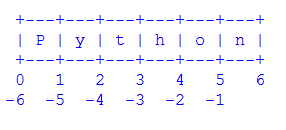
\includegraphics[scale=1]{string-slicing.png}
\caption{String slicing}
\end{figure} 

\textbf{Note:} Indexing a string that is out of range gives an error. But when slicing it doesn't give and error but the maximum number is replaced with the out of range word.

\texttt{\\
>>> word = 'Python'\\
>>> word[0]\\
'P'\\
>>> word[-1]\\
'n'\\
>>> word[0:2] \# This can also be written as word[:2]\\
'Py'\\
>>> word[0:2] + word[2:]\\
'Python'\\
>>> word[42]\\
IndexError:\\
>>> word[4:42]\\
'on'
}
\subsection{Unicode Strings}
Unicode strings are supported in python. They follow the \texttt{http://unicode.org} rules. With the help of unicode strings we can display any non ascii code or any string which is not a 8-bit string. If we place \texttt{'u'} in front of the string it means to python that a unicode string is being created. We can also convert them using the \texttt{string.encode(encoding)}. \texttt{unicode(string,encoding)} will convert unicode characters to original characters.
\texttt{\\
>>> text = u'ä'\\
u'$\setminus$xe4'\\
>>> \# To print the value we will use the 'print'\\
>>> print text\\
ä\\
>>> u"ä".encode(utf-8)\\
'$\setminus$xe4'\\
>>> unicode('$\setminus$xe4',utf-8)\\
ä
}

\subsection{Strings - Miscellaneous}
\begin{itemize}
\item Strings are immutable in python.It means that they cannot be changed once they are created. We will have to create them again if we have any problem.
\item len(string) will give the length of the string.
\end{itemize}
\texttt{
>>> word[1] = 'J'\\
TypeError:\\
>>> len(word)\\
6
}
\section{Lists}
Lists in python are like string objects. They can be \textbf{indexed, sliced, concatenated}. But the biggest difference between strings and lists is that they are mutable. That is they can be changed. We can use the \texttt{append} method to add an item to the lists. We can even define new values to the slices which are in the given range. Using slices we can also change the length of the lists. We can find the length of the lists using the \texttt{len} function. Finally \textbf{lists can be nested} one in another.
  
\texttt{\\
>>> lis = [1,2,3,4,5]\\
>>> lis[1]\\
2\\
>>> lis[$:$2]\\
{[1,2]}\\
>>> new\_list = lis[$:$3]+[9,8,7]\\
>>> new\_list = [1,2,9,8,7]\\
>>> new\_list[2$:$5] = []\\
>>> new\_list.append(3)\\
>>> new\_list[2] = 5\\
>>> len(new\_list)\\
3\\
>>> nested\_list = [1,2,3,4,5,6,[7,8,9]]\\
}



\section{If elif else statements}
In python \texttt{if...elif..elif...else} statements are same as they are in other languages. Here \texttt{elif} is same as \texttt{else} if in othe languages. In python there is no switch statements. 

\texttt{\\
>>> x = int(raw\_input('Please enter an integer: '))\\
Please enter an integer: 42\\
>>> if x < 0:\\
...\hspace{30pt}x = 0\\
...\hspace{30pt}print "The number you have entered is negative"\\
...elif x == 0:\\
...\hspace{30pt}print "Zero"\\
...elif x == 1:\\
...\hspace{30pt}print "Single"\\
...else:\\
...\hspace{30pt}print "More"\\
...\\
More
}



\section{For Loops}
In python for loops are not like in other programming languages. Here for loops iterate over a sequence like lists, strings, tuples and few other objects. \textbf{If we want to make a modification to any list using for loop, then it is advised to use the slicing otherwise the program becomes infinite and keeps on adding to the list and iterating over the same object.(Program 2)}.


\texttt{\\
>>> \# Program 1\\
>>> words = ['cat','dog','snake']\\
>>> for w in words:\\
...\hspace{30pt}print w, len(w)\\
...\\
cat 3\\
dog 3\\
snake 5\\
\\
>>> \# Program 2\\
>>> for w in words[:]:\\
...\hspace{30pt}if len(w)>4:\\
...\hspace{30pt}\hspace{30pt}words.insert(0,w)\\
...\\
>>> words\\
{['snake','cat','dog','snake']}\\
\\
>>> \# Program 3 - The program with problem\\
>>> for w in words:\\
...\hspace{30pt}if len(w)>4:\\
...\hspace{30pt}\hspace{30pt}words.insert(0,w)\\
...\hspace{30pt}\hspace{30pt}print "Insert One now!"\\
...\\
This is causing an infinite program to be created.\\
}

In program 2 we are not actually using the words list directly but we are indirectly creating a copy of the same and then looping over it. Thus the program prints only limited number of times and not unlimited number of times. \textbf{This problem is only if we are modifying the list and using the same list for iteration}

\subsection{Range Function}
Range function is an inbuilt function. This function will generate numbers in the given range and in a sequence as like in the traditional c language style. Range function is of three types.\\
\begin{itemize}
\item \texttt{range(stop)} - Starts from 1, ends at 'stop', with a 'step' of 1.
\item \texttt{range(start,stop)} - starts at 'start', stops at 'stop', with a step of 1.
\item \texttt{range(start,stop,step)} - starts at 'start', stops at 'stop', with a step of 'step'.
\end{itemize}

\texttt{
\\
>>> for i in range(5,11,2):\# It doesn't take into consideration 11\\
...\hspace{30pt}print i\\
...\\
5\\
7\\
9\\}

\subsection{Break and continue statements}
\texttt{break} statements in loops are like the same in the traditional C language. When a break statement is encountered in a loop the loop stops executing at that moment and exits the loop. In the similar way \texttt{continue} statement is used to exit the current iteration and continue the looping process as it is.

\texttt{
\\
>>> \# Program 1\\
>>> for i in range(2,10):\\
...\hspace{30pt}if num\%2 == 0:\\
...\hspace{30pt}\hspace{30pt}print "Found an even number ",num\\
...\hspace{30pt}\hspace{30pt}continue\\
...\hspace{30pt}print "Found a number ",num\\
...\\
Found an even number 2\\
Found a number 3\\
Found an even number 4\\
Found a number 5\\
Found an even number 6\\
Found a number 7\\
Found an even number 8\\
Found a number 9\\
\\
>>> \# Program 2\\
>>> for i in range(2,10):\\
...\hspace{30pt}if num\%2 == 0:\\
...\hspace{30pt}\hspace{30pt}print "Found an even number ",num\\
...\hspace{30pt}\hspace{30pt}break\\
...\hspace{30pt}print "Found a number ",num\\
...\\
Found an even number 2\\
>>> \# Program breaks after first iteration as it encounters the break statement.
}

\subsection{Else Statement of loops}
In python \texttt{else} statement is executed after the loop is finished with the items in the list. But the else statement is not executed when the loop breaks out with the \texttt{break} statement. To be simple using else statements with \texttt{for \& while} is like \texttt{do...while} in C programming.

\texttt{
\\
>>> for n in range(2,10):\\
...\hspace{30pt}for x in range(2,n):\\
...\hspace{30pt}\hspace{30pt}if n\%x == 0:\\
...\hspace{90pt}print n, 'equals',x,'*',n/x\\
...\hspace{90pt}break\\
...\hspace{30pt}else:\\
...\hspace{60pt}\# loop fell through without finding a factor\\
...\hspace{60pt}print n,'is a prime number'\\
2 is a prime number\\
3 is a prime number\\
4 equals 2 * 2\\
5 is a prime number\\
6 equals 2 * 3\\
7 is a prime number\\
8 equals 2 * 4\\
9 equals 3 * 3\\
}

\subsection{Pass statement}
Pass statement is a dummy statement and it is like a comment in python. It is used when there should be a statement syntactically but the program should not do any action. This can be used when we are in the abstract level in starting a very complicated program with complicated algorithm.

\texttt{
\\
>>> if anivarth == "peesapati"\\
...\hspace{30pt}pass\\
...\\
>>>\\}
\section{While loop}
While loop is similar to for loop but here it checks the condition and doesn't iterate like for loop over lists. All the above subsections(7.2-7.4) are usable with while statement.
\texttt{\\
>>> count = 0\\
>>> while count<6:\\
...\hspace{30pt}print count,\\
...\hspace{30pt}count = count+1\\
...\\
0$\:$1$\:$2$\:$3$\:$4$\:$5\\
>>> \# ',' after the print statement prints the next print in the same line}



\section{Functions}
\texttt{def} is used to define a function. The word after the def keyword is the name of the function. Parameters are the parenthesized list of variables. Next line following the definition of the function contains the \textbf{function body}. If we add a string lateral to the first line of the function then it becomes \textbf{docstring}. It is used for documentation of the function.

\texttt{\\
>>> def fib(n): \#Write fibonacci series upto n\\
...\hspace{30pt}"""Print a Fibonacci series upto n."""\\
...\hspace{30pt}a, b = 0, 1\\
...\hspace{30pt}while a < n:\\
...\hspace{30pt}\hspace{30pt}print a,\\
...\hspace{30pt}\hspace{30pt}a,b = b, a+b\\
...\\
>>> fib(10)\\
0$\:$1$\:$1$\:$2$\:$3$\:$5$\:$8\\
>>> fib.\_\_doc\_\_\\
'Print a Fibonacci series upto n.'
} 

Usually a function without a return statement is called a \textbf{procedure}. But python function returns \texttt{None} object when there is no return statement. Thus procedures in python can be called as functions.

\subsection{Variable scope}
When a function is executed a new \textbf{symbol table} is created for storing the local variables. When referencing a variable python first searches in the local symbol table, then local symbol table of enclosing functions, next in the global symbols table and finally in the built-in names. \textbf{If we assign a new value to a variable that has already been defined outside the enclosing function, a new symbol is created in the local symbol table and the real value of the variable in the global symbol table doesn't change eventhough we use the same name.} The arguments that we pass in the function definition, new variables are created in the local symbols table and then they are used(\textbf{i.e. Arguments are passed using call by value}). When function is created a new symbol is created in the current symbol table. The value of the function name has \texttt{type} function.

\texttt{\\
>>> a = 15\\
>>> def funct():\\
...\hspace{30pt}a = 10\\
...\\
>>> funct()\\
>>> a\\
15\\
>>> \# Even though we have changed the value of 'a' in the function the value didn't change in the global variable\\
>>> \# Argument values are stored in the local symbol table before used.\\
>>> def functi(d):\\
...\hspace{30pt}d = 500\\
...\\
>>> functi(a)\\
>>> a\\
15\\
>>> type(functi)\\
<type 'function'>\\
>>>
}


\subsection{Default argument values in python}
We can even define functions with the argument values already defined. With this we can call the function with fewer arguments. \textbf{Argument values are defined at the point of function definition(Program 2). Default values are evaluated only once(Program 3).}

\texttt{\\
>>> \# Program 1\\
>>> def ask\_ok(prompt, retries =4, complaint = 'Yes or no, Please!'):\\
...\hspace{30pt}while True:\\
...\hspace{30pt}\hspace{30pt}ok = raw\_input(prompt)\\
...\hspace{30pt}\hspace{30pt}if ok in ('y','ye','yes')\\
...\hspace{30pt}\hspace{30pt}\hspace{30pt}return True\\
...\hspace{30pt}\hspace{30pt}if ok in ('n','no','nop','nope'):\\
...\hspace{30pt}\hspace{30pt}\hspace{30pt}return False\\
...\hspace{30pt}\hspace{30pt}retries = retries - 1\\
...\hspace{30pt}\hspace{30pt}if retries < 0:\\
...\hspace{30pt}\hspace{30pt}\hspace{30pt}raise IOError('refusenik user')\\
...\hspace{30pt}\hspace{30pt}print complaint\\
...\\
>>> \\
>>> \# Program 2\\
>>> i = 5\\
>>>\\
>>> def f(arg=i):\\
...\hspace{30pt} print arg\\
...\\
>>> i = 6\\
>>> f()\\
5\\ 
>>> \\
>>> \# Program 3\\
>>> def f(a,L=[]):\\
...\hspace{30pt}L.append(a)\\
...\hspace{30pt}return L\\
...\\
>>> print f(1)\\
{[1]}\\
>>> print f(2)\\
{[1,2]}\\
>>> print f(3)\\
{[1,2,3]}\\
>>>\\
}

The above function(program 1) can be called in three different ways.
\begin{itemize}
\item Giving only the mandatory value: \texttt{ask\_ok('Do you really want to quit?')}
\item Giving one optional argument: \texttt{ask\_ok('Do you really want to quit?',2)}
\item Giving more than two arguments: \texttt{ask\_ok('Do you really want to quit?',2,'Come on, only yes or no!')}
\end{itemize}


\subsubsection{Keyword Arguments}
If we define a function then the keyword arguments calls should follow the conditions:
\begin{itemize}
\item Should not miss required argument.
\item Directly define the value of the non keyword argument after a keyword argument.
\item Defining the same argument twice.
\item Defining the value to a non key word argument.
\end{itemize}

For Instance we have defined a function: \\ \texttt{def parrot(voltage,state='alive',action='voom',type='Norwegian'}, then the following usage should not happen\\
\texttt{\\
>>> parrot() \# Required keyword missing\\
Error:\\
>>> parrot(voltage=5.0,'dead') \# non-keyword argument after a keyword argument.\\
Error:\\
>>> parrot(110,voltage=220) \#duplicate value for the same argument.\\
Error:\\
>>> parrot(actor="John Cleese") \# Unknown argument.\\
Error:\\
>>> \\
\\
}
In a function call, keywords arguments must follow positional arguments. All the keyword  arguments passed must match one of the arguments accepted by the function an their order is not important. This also includes non-optional arguments. NO argument may receive a value more than once. 

\subsection{Arbitary Argument values}
Sometimes there will be a situation when we don't know what value the user will enter. We can use \texttt{*args} and \texttt{**kwords} like format to specify python that the user is going to enter a list and dictionary respectively. We can use any one of them. To be specific \texttt{*args} takes tuple as input and **kwords takes dictionary as input. 
\texttt{\\
>>> def cheeseshop(kind,*arguments,**keywords):\\
...\hspace{30pt} print "-- Do you have any",kind,"?"\\
...\hspace{30pt} print "-- I'm sorry, we're all out of",kind\\
...\hspace{30pt}for arg in arguments:\\
...\hspace{30pt}\hspace{30pt}print arg\\
...\hspace{30pt}print "-"*40\\
...\hspace{30pt}keys = sorted(keywords.keys())\\
...\hspace{30pt}for kw in keys:\\
...\hspace{60pt}print kw, ":",keywords[kw]\\
...\\
}
\\
\textbf{As we know that range function takes tuples as input we can give input to the range function the arbitrary argument values \texttt{*args} to unpack it.}\\
\texttt{>>> arg = [3,6]\\
>>> range(*arg)\\
{[3,4,5]}\\
>>>
}

\subsection{Documentation strings}
When a function is created its documentation is really important. But python suggests some of the rules that can be followed if desired. This will make the documentation simple for others to use it. 
\begin{itemize}
\item The first line in the multi line string should have a very small brief introduction to what the function does followed by a period.  The second line should be blank. Third line should have all the details of any side effects using this function has. If there are no side effects then this can be skipped and be replaced with the usage of the function and object calling conventions. You can add all the required arguments, optional arguments and few other things here.
\end{itemize}

\texttt{\\
>>> def func():\\
...\hspace{30pt}""" This line has been added for the sake of documenting the function.\\
...\hspace{30pt}\\
...\hspace{30pt}This function "does nothing" to harm your computer."""\\
...\hspace{30pt}pass\\
...\\
>>> print func.\_\_doc\_\_\\
This line has been added for the sake of documenting the funciton.\\
\linebreak
.\hspace{30pt}This function "does nothing" to harm your computer.
}


\section{Lambda expressions}
Lambda expressions are used to create anonymous functions  at  a given point of the code. Anonymous functions are the functions which doesn't have any name.  They are useful when the function is used for the once like in \textbf{a} for loop or while loop or filter or map etc.

\texttt{\\
>>> foo = [2,18,9,22,17,24,8,12,27]\\
>>> \# Now we will create an anonymous function.\\
>>> print filter(lambda x:x\%3 == 0, foo)\\
{[18,9,24,12,27]}\\
>>> def f(x): return x**2\\
...\\
>>> print f(8)\\
64\\
>>>\\
>>> g = lambda x: x**2\\
>>>\\
>>> print g(8)\\
64\\
>>>
}

\section{Python coding style: PEP8}
PEP 8 has emerged has a style guide for python. It is recommended to use PEP 8 styles so that the program is easy to use and can be used by any one in the world without any problem. Some of the key points in PEP 8 are as follows:
\begin{itemize}
\item Use 4-space indentation, and no tabs.
\item Wrap lines so that they don’t exceed \textbf{79 characters}.
\item Use blank lines to separate functions and classes, and larger blocks of code inside functions.
\item When possible, put comments on a line of their own.
\item Use docstrings.
\item Use spaces around operators and after commas, but not directly inside bracketing constructs: \texttt{a = f(1, 2) + g(3, 4).}
\item Name your classes and functions consistently; the convention is to use \texttt{CamelCase} for classes and \texttt{lower\_case\_with\_underscores} for functions and methods. Always use \texttt{self} as the name for the first method argument.
\item Don’t use fancy encodings if your code is meant to be used in international environments. Plain ASCII works best in any case. 
\end{itemize}

\section{Data Structures}
In this section we will discuss more on lists, tuples, dictionaries and few other things.
\subsection{More on lists}
\begin{itemize}
\item \texttt{a.count(x)} - Count the number of instances \texttt{x} has appeared in the list a.
\item \texttt{a.insert(i,x)} - Insert \texttt{x} at i in the list a.
\item \texttt{a.append(x)} - Insert \texttt{x} at the end of the list a.
\item \texttt{a.index(x)} - Find the place of first instance of \texttt{x} in the list a.
\item \texttt{a.remove(x)} - Remove the first instance of \texttt{x} in the list a.
\item \texttt{a.reverse()} - Reverse the given list a.
\item \texttt{a.sort(cmp=None, key=None, reverse=False)} - Sort the list in ascending order if the default is used without any arguments and if reverse is specified as \texttt{True}, then the list is sorted in descending order. More about the arguments in the \texttt{sorted()} function.
\item \texttt{a.pop([i])}\footnote{Square brackets in the documentation of a function represents that the argument is optional to be entered.} - Remove the given argument \texttt{i} and return the removed element if the argument is specified or else remove the last element and return the last element of the list a. 
\end{itemize}
It should be noted that the return values of the functions like \texttt{sort, remove, insert} which don't return anything is \texttt{None}. \\
\texttt{
\\
>>> a = [66.25,333,333,1,1234.5]\\
>>> print a.count(333), a.count(66.25),a.count('x')\\
2 1 0\\
>>> a.insert(2,-1)\\
>>> a.append(333)\\
>>> a\\
{[66.25, 333, -1, 333, 1, 1234.5, 333]}\\
>>> a.index(333)\\
1\\
>>> a.remove(333)\\
>>> a\\
{[66.25, -1, 333, 1, 1234.5, 333]}\\
>>> a.reverse()\\
>>> a\\
{[333, 1234.5, 1, 333, -1, 66.25]}\\
>>> a.sort()\\
>>> a\\
{[-1, 1, 66.25, 333, 333, 1234.5]}\\
>>> a.pop()\\
1234.5\\
>>> a\\
{[-1, 1, 66.25, 333, 333]}\\
>>>\\ }
\subsubsection{Using lists as stacks}
LIFO (Last In-First out) can be done using the \texttt{append \& pop} methods. Add the element to top of  the stack(list) using the \texttt{append} and then remove the top element of the stack(list) using the \texttt{pop} method.
\texttt{\\
>>> stack = [1,2,3]\\
>>> stack.append(4)\\
>>> stack.append(5)\\
>>> stack.pop()\\
5\\
>>> stack.pop()\\
4\\
>>>
}
\subsubsection{Using lists for queues}
In a queue a person who has entered first will be the first to leave. Also called as FIFO(First In First Out). While we can use the \texttt{append} and the \texttt{remove} method to remove the element from the list this becomes inefficient. So it is better to use the \texttt{collections.deque} from the \texttt{collections} module. 

\texttt{\\
>>> from collections import deque\\
>>> queue = deque(["Eric","John","Michael"])\\
>>> queue.append("Terry")\\
>>> queue.append("Graham")\\
>>> queue.popleft()\\
'Eric'\\
>>> queue.popleft()\\
'John'\\
>>> \\ }
We can also use the combination of \texttt{reverse,pop}, with functions to do the same task.
\subsubsection{\texttt{filter} function}
\texttt{filter} function is used to filter the values in a list. Calling \texttt{filter(function, list)} will return the value in the list for which the \texttt{function(item)} is true. If the result is a \texttt{string, tuple} the result will be string or tuple otherwise the result will be always a \texttt{list}.

\texttt{\\
>>> def f(x): return x\%3 == 0 or x\%5 == 0\\
...\\
>>> filter(f, range(2,25)) \# We should not put \texttt{()} for the function name.\\
{[3, 5, 6, 9, 10, 12, 15, 18, 20, 21, 24]}\\
>>>\# We can also use the lambda instead of defining the function\\
 >>> filter(lambda x:x\%3 ==0 or x\%5 ==0, range(2,25))\\
{[3, 5, 6, 9, 10, 12, 15, 18, 20, 21, 24]}\\
>>>}
\subsubsection{\texttt{map} function}
\texttt{map} function is used to map the values of the list to the function. \texttt{map(function name, list)} will return a list containing the values of \texttt{function(item)}.

\texttt{\\
>>> map(lambda x:x**3, range(1,11))\\
{[1, 8, 27, 64, 125, 216, 343, 512, 729, 1000]}\\
}\\
We can also pass more than one sequence where the values of both the sequences usage is needed. Here we cannot use lambda because \texttt{lambda} will only take one input argument and we cannot give more than one argument. \texttt{lambda x:x**3}, \cancel{\texttt{lambda a:b+c}}\\
\texttt{\\
>>> map(add, range(8),range(8))\\
{[0, 2, 4, 6, 8, 10, 12, 14]}\\
}\\
\textbf{Note}: We cannot use \texttt{range(x,y)} inside a map function because of the '\textbf{,}' \texttt{map} thinks that the parameter of the next sequence is given and raises an error. But this is \textbf{not} the case in \textbf{filter function}
\subsubsection{\texttt{reduce} function}
\texttt{reduce} function will take the first two values of the sequence and will send it to the function, in the next section it will call the result of first two with the third one and so on. It is like using fibonaccii sequence.
\texttt{\\
>>> def add(x,y): return x+y\\
...\\
>>> reduce(add, range(1,10))\\
45\\
}

\textbf{Note}: If an empty sequence is given as input an error is raised. For that we will add a third argument which indicates the starting value and will not raise any exception.

\texttt{\\
>>> reduce(add,range(0))\\
Error:\\
>>> reduce(add,range(0),0)\\
0}
\subsection{List Comprehension}
We can create or change the items in the lists in a simple and easy way using list comprehensions. The sequence to create list comprehension is a for loop followed by a for loop which is optional and followed by a if conditional which is again optional. We can create a two element tuple. But when we create a tuple the values should be parenthesized otherwise the interpreter will raise an exception.

\texttt{\\
>>> vec = [-4,-2,2,4]\\
>>> \#Crate a new list with the values doubled\\
>>> [x*2 for x in vec]\\
{[-8, -4, 4, 8]}\\
>>> \#filter the list to exclude negative numbers\\
>>> [x for x in vec if x>=0]\\
{[2, 4]}\\
>>> \#Apply a function to all the elements\\
>>> [abs(x) for x in vec]\\
{[4, 2, 2, 4]}\\
>>> \#call a method on each element\\
>>> freshfruits = ['  banana','loganberry  ','passion fruit  ']\\
>>> [weapon.strip() for weapon in freshfruits]\\
{['banana', 'loganberry', 'passion fruit']}\\
>>> \# Create a list of 2 tuples like (numbers,squares)\\
>>> [(x,x**2) for x in range(6)]\\
{[(0, 0), (1, 1), (2, 4), (3, 9), (4, 16), (5, 25)]}\\
>>> \#The tuple must be parenthesized, otherwise an error will occur\\
>>> [x,x**2 for x in range(6)]\\
SyntaxError: invalid syntax\\
>>> vec = [[1,2,3],[4,5,6],[7,8,9]]\\
>>> [num for elem in vec for num in elem]\\
{[1, 2, 3, 4, 5, 6, 7, 8, 9]}\\
>>> \\
}
\subsubsection{Nested list comprehensions}
There can also be nested list comprehensions. i.e. we can add comprehension in a comprehension. 

\texttt{\\
>>> matrix = [\\
...\hspace{30pt}{[1,2,3,4]},\\
...\hspace{30pt}{[5,6,7,8]}\\
...\hspace{30pt},{[9,10,11,12]]}\\
>>> matrix\\
{[[1, 2, 3, 4], [5, 6, 7, 8], [9, 10, 11, 12]]}\\
>>> [[row[i] for row in matrix] for i in range(4)]\\
{[[1, 5, 9], [2, 6, 10], [3, 7, 11], [4, 8, 12]]}\\
>>> \\
}
\subsection{\texttt{del} statement}
\texttt{del} statement is used to delete an item in the list or even the slices using the index. We can also delete a variable using the del statement. This is different from the \texttt{pop} method because the \texttt{pop} method returns the removed element.

\texttt{\\
>>> dell = [1,2,3,4,5,6]\\
>>> del dell[1]\\
>>> dell\\
{[1, 3, 4, 5, 6]}\\
>>> del dell[1:3]\\
>>> dell\\
{[1, 5, 6]}
>>> del dell\\
>>> dell\\
Error: Traceback error, Varaible name not defined\\
>>> \\}

\subsection{Tuples}
Tuples are \textbf{immutable} object which is an another type of sequence data. We can perform operations like indexing, slicing operations the same way as we have done in lists and strings. Tuples are defined by a number of values separated by comma.   Tuples are always nested by parenthesis. Although while defining it is not really necessary, but it will be better if we use the parenthesis for defining tuples. 

Empty tuples are constructed by using an empty pair of parenthesis, but a single valued tuple is constructed using the value followed by a comma with parenthesis surrounding it.

\texttt{\\
>>> t = 12345,54321, 'hello!'\\
>>> t[0]\\
12345\\
>>> t\\
(12345, 54321, 'hello!')\\
>>> \#Tuples may be nested:\\
>>> u = t, (1,2,3,4,5)\\
>>> u\\
((12345, 54321, 'hello!'), (1, 2, 3, 4, 5))\\
>>> \#Tuples are immutable\\
>>> t[0] = 88888\\
TypeError: 'tuple' object does not support item assignment\\
>>> \#but they can contain mutable objects:\\
>>> v = ([1,2,3],[3,2,1])\\
>>> v\\
([1, 2, 3], [3, 2, 1])\\
>>> empty = ()\\
>>> singleton = 'hello',\\
>>> len(empty)\\
0\\
>>> len(singleton)\\
1\\
>>> singleton\\
('hello',)\\
>>>\\ }

\subsubsection{Difference between tuples and lists}
One would say the main difference between a tuple and list is they are enclosed by parenthesis and square brackets respectively. But there is a very big difference. Tuples are immutable and lists are mutable. i.e. we cannot changed the once assigned values in tuples but we can do so in lists. Tuples are heterogeneous objects and lists are homogeneous objects. Heterogeneous means that the values which we enter in tuples does have a relation to each other but they are some other type. For example Hours and minutes in time have relation with each other but they are different. While lists have some relation to each other and they are of same type. It should be noted here that the heterogeneity and homogeneity is only in the data which exists in the real world and not in the data type we enter in the lists or tuples. Of course we can enter different data types(like \texttt{int, strings, etc.}) even in lists also. Also a misconception is that tuples are some constant lists. But if they were lists(constant or not) then we could have changed the elements in them. A big difference comes in terms of their routine usage. This has been stated in python documentation. Elements in tuple are accessed by unpacking or indexing and the elements in lists are accessed by iterating over the list. We can even perform unpacking using lists but it is not usually done like that, but when unpacking is used on lists we will have to specify the square brackets and this is not required in case of tuples. To be simple unpacking is the usage of \texttt{x,y,z = t} where t is already defined. The only condition for performing unpacking is that the number of variables used on the left hand side should be equal on the right side. See the code to understand more.

\texttt{\\
>>> tup = (1,2,3)\\
>>> lis = [1,2,3]\\
>>> tup(2) = 10\\
Error:\\
>>> lis(2) = 5\\
>>> lis\\
{[1,2,5]}
>>> tup1 = (2016,1,26)\\
>>> lis1 = [1,2,3,4,5]\\
>>> tup2 = ('anivarth',20)\\
>>> lis2 = ('anivarth','peesapati')\\
>>>\\
>>>\# Example on unpacking\\
>>> t = (1,2,3)\\
>>> x,y,z = t\\
>>> x\\
1\\
>>> \# The above can also be done on lists but it is not usually used. An example is:\\
>>> [x,y,z] = [1,2,3] \# We can also assign it to a tuple
}\\
\textbf{References:} \texttt{http://ow.ly/Xr8W3 , http://ow.ly/Xr8Ze, http://ow.ly/Xr91U}\\

\subsection{Sets in python}
Python also supports the sets which we use in mathematics. We can perform union, itersection, difference etc. Basically sets are a collection of objects which don't have any duplicates and they are unordered collection. But remember that they can also be ordered. Here unordered means that the position of the element is not really important.
A set can be created using \texttt{$\lbrace\rbrace$} or using \texttt{set()}, but for empty set we will have to use \texttt{set()}. Usage of \texttt{$\lbrace\rbrace$} without anything will create a dictionary. Also list comprehension can be used with sets.

\texttt{\\
>>> basket = ['apple','orange','apple','pear','orange','banana']\\
>>> fruit = set(basket)\\
>>> fruit\\
set(['orange', 'pear', 'apple', 'banana'])\\
>>> 'orange' in fruit\\
True\\
>>> \# Demonstrate set operations on unique letters from two words\\
>>> a = set('abracadabra')\\
>>> b = set('alacazam')\\
>>> a\\
set(['a', 'r', 'b', 'c', 'd'])\\
>>> a-b\\
set(['r', 'b', 'd'])\\
>>> a|b\\
set(['a', 'c', 'b', 'd', 'm', 'l', 'r', 'z'])\\
>>> a\&b\\
set(['a', 'c'])\\
>>> a\textasciicircum b\\
set(['b', 'd', 'm', 'l', 'r', 'z'])\\
>>> a = $\lbrace$'fruit','hello'$\rbrace$\\
>>> a\\
set(['fruit', 'hello'])
>>> a = $\lbrace$x for x in 'abracadabra' if x not in 'abc'$\rbrace$\\
>>> a\\
set(['r', 'd'])\\
>>> \\
}
\subsection{Dictionaries in python}
Dictionaries in python are also sequences which are like lists. But unlike lists dictionaries will use keys to refer to its elements. The condition is that the type of keys should be immutable type like strings and numbers. Tuples can also be used for the keys but they should only contain strings and numbers but not lists because lists are mutable. Also lists cannot be used directly as keys because they are mutable. 
Dictionaries are unordered set of key:value pairs. We can create dictionary using \texttt{$\lbrace\rbrace$} and also using \texttt{dict()}. Using \texttt{dict()} we can pass tuples for creating dictionary. We can also connect the key value pairs using \texttt{=} to create dictionary using \texttt{dict()}.  All the key value pairs are separated using a comma. We cannot add two key value pairs with the same key name. If it is done then the new one will replace the old one. The main advantage of dictionaries over lists is that we can name each element based on requirement. We can also use \texttt{del} to delete the corresponding key value pair.  To get  a list of all the keys in the given dictionary we can use \texttt{.keys()} method. And they are also unordered. i.e. even if we both enter the same dictionary at the same time it is not guaranteed that we get the same list if we apply the \texttt{.keys()} method. To check a single key we use \texttt{in} keyword. List comprehension is also valid for dictionary.

\texttt{\\
>>> tel = $\lbrace$'jack'{:}4098,'sape'{:}4139$\rbrace$\\
>>> tel['guido'] = 4127\\
>>> tel\\
$\lbrace$'sape'{:}4139, 'jack'{:}4098, 'guido'{:}4127$\rbrace$\\
>>> tel['jack']\\
4098\\
>>> del tel['sape']\\
>>> tel[5] = 5698\\
>>> tel['irv'] = 4127\\
>>> tel\\
$\lbrace$5{:} 5698, 'jack'{:} 4098, 'irv'{:} 4127, 'guido'{:} 4127$\rbrace$\\
>>> tel.keys()\\
{[5, 'jack', 'irv', 'guido']}\\
>>> 'guido' in tel\\
True\\
>>> dict([('sape',4139),('guido',4127),('jack',4098)])\\
$\lbrace$'sape'{:}4139, 'jack'{:}4098, 'guido'{:}4127$\rbrace$\\
>>> $\lbrace$x{:}x**2 for x in (2,4,6)$\rbrace$\\
$\lbrace$2{:}4, 4{:}16, 6{:}36$\rbrace$\\
>>> dict(sape=4139, guido=4127, jack=4098)\\
$\lbrace$'sape'{:}4139, 'jack'{:}4098, 'guido'{:}4127$\rbrace$\\
>>> }
\section{Techniques in looping}
As we have many types of sequences we also have many techniques in looping also. While looping in a \textbf{sequence} to get the index and the corresponding value can be obtained by using \texttt{enumerate()} function. The enumerate function actually returns the values in the form of tuples. (Program 1). To iterate over two sequences or more at a time then we will use \texttt{zip} function which will print $i^{th}$ element of each list in a tuple.(Program 2). Note that if the zip element is supplied with two lists of different sizes then it will iterate the lowest number of elements list size times.  We can also use \texttt{xrange(start, stop, step)}, to generate a sequence of numbers the same way \texttt{range} generates the sequence. But \texttt{range \& xrange} differ mainly in two aspects. 1. \texttt{range} generates a list object but \texttt{xrange} generates xrange object. 2. \texttt{xrange} uses a technique called \emph{yielding} to generate the sequence and this will be very efficient when we will use it in very small memory devices like phone. Also this will use very memory when generating very long iterations like billions and billions. While the \texttt{range} will use almost the whole memory it can use.\\
Reference: \texttt{http://goo.gl/hKZUIt}

\texttt{\\
>>> \# Program 1\\
>>> for i, v in enumerate(['tic','tac','toe']):\\
...\hspace{30pt}print i,v\\
...\\
0 tic\\
1 tac\\
2 toe\\
>>> \# Program 2\\
>>> for i,v in zip(range(2),range(100)):\\
...\hspace{30pt}print i,v\\
...\\
0 0\\
1 1\\
>>> \\
>>> \# Using xrange\\
>>> for i in reversed(xrange(3)):\\
...\hspace{30pt}print i\\
...\\
2\\
1\\
0\\
}

When iterating over a dictionary we can use \texttt{.iteritems()} method to generate tuples of key value pairs.

\texttt{\\
>>> knights = $\lbrace$'gallahad':"the pure",'robin':'the brave'$\rbrace$\\
>>> for k,v in knights.iteritems():\\
...\hspace{30pt}print k, v\\
...\\
gallahad the pure\\
robin the brave\\
>>>
}
\section{Conditions and comparisions}
All the comparison operators like \texttt{==, <, >, <=, >=, in, not in, is, not is} have same priority which is less than the mathematical operators priority. i.e. mathematical operations are performed first when compared to comparisons. Here, \texttt{in \& not in} check whether the value occur or doesn't occur in a sequence and \texttt{is \& not is}  check whether the given two elements are same or not. 

\texttt{\\
>>> a = 'a'\\
>>> 'a' is a\\
True\\
>>> anivarth = 'peesapati'\\
>>> 'peesa' in anivarth\\
True\\
>>>\\}

Comparisons can be combined with boolean operators \texttt{and \& or}. It should be remembered that the priority of boolean operators is less than that of comparison operators. While in boolean \texttt{not} has the highest priority and \texttt{or} has the lowest priority.

It should be noted that the comparisons in sequences follow lexicographical ordering. i.e. the first element in list one is compared to first element in second list and if it is true then the second elements are compared. \textbf{Comparing two different data types has the outcome to be deterministic but it is arbitrary}

\section{Modules}
To use the functions and the definitions again and again we define them in a script called as module. We can import the definitions and functions into other modules or into the main module. A module is a file name with the suffix \texttt{.py} . Within a module its name is available as \texttt{\_\_name\_\_}.  Saving the following file as \texttt{fibo.py}.

\begin{verbatim}
# Fibonacci numbers modules
def fib(n): #write fibonacci series up to n
    a, b = 0,1
    while b<n:
        print b,
        a, b = b, a+b
    
def fib2(): #return Fibonacci series up to n
    result = []
    a, b = 0, 1
    while b < n:
        result.append(b)
        a, b = b, a+b
    return result
\end{verbatim}
To run this script from somewhere else we will have to import the \texttt{sys} module and append the path of the module location to it. We are doing this because, when a module is executed python first searches for directories given by the path \texttt{sys.path}. \texttt{sys.path} searches in this manner.
\begin{itemize}
\item Directory containing the module or the script.
\item \texttt{PYTHONPATH}. Directories with same syntax and same as the shell \texttt{PATH}.
\item the installation dependent default.
\end{itemize}

\begin{verbatim}
>>> import sys
>>> sys.path.append('C:\\users\\sekhar peesapati\\desktop\\python notes')
>>> import fibo
>>> fibo.fib(3)
1 1 2
>>> fibo.__name__
'fibo'
\end{verbatim}
\subsection{More on modules}
Each module has its own private symbol table, which is used as the global symbol table by all functions defined in the module. With this the author of the module need not worry that the names will clash with the names in the main global symbol table. \textbf{It is good practice to place all the import statements in the beginning of the code.} We can also use the \texttt{*} to import all the names in the module but this will \textbf{not import the names beginning with \texttt{\_}}

\begin{verbatim}
>>> from fibo import fib, fib2
>>> fib(500)
1 1 2 3 5 8 13 21 34 55 89 144 233 377
\end{verbatim}

\subsubsection{Executing modules as scripts}
When we will run the python script as main program then python sets \texttt{\_\_name\_\_} to \texttt{'\_\_main\_\_'}. For example if we are running the script in a command prompt and we are getting the arguments then we can add the following code, so that if the user uses the script as module then the \texttt{\_\_name\_\_} is set to the name of the module and the code under the if block doesn't run.
\begin{verbatim}
def add(x):    print x+10

if __name__ == __main__:
    import sys
    add(int(sys.argv[1]))
\end{verbatim}  

Executing the above code will give the result as follows:
\begin{verbatim}
$ python add.py 50
60
\end{verbatim}


\subsection{Compiled python files}
Compied python files are saved as \texttt{.pyc} files. These files are created when we will compile the python program and if the error occurs in compiling the \texttt{.pyc} file is treated as invalid. 

These \texttt{.pyc} files help us when we will use the same module for the next time. This time python checks whether the created \texttt{.pyc} file has the same modification time as the corresponding \texttt{.py} file, if yes it will use it otherwise it is ignored. 

\texttt{.pyc} files doesn't help program run more faster they only help in loading the module faster. Also these files are hard to reverse engineer so that the contents in the file can be distributed safely.

\subsection{Standard Modules, \texttt{dir()} and \texttt{\_\_builtin\_\_}}
Python comes with some standard modules which have their own functionality. But a few come along with the interpreter so that the os specific files can be distributed only to the required os. One example worth mentioning is the \texttt{sys} module an its usage in the command prompt is as follows:
\begin{verbatim}
>>> import sys
>>> sys.ps1
'>>> '
>>> sys.ps2
'... '
>>> sys.ps1 = 'anivarthIsGreat>>> '
anivarthIsGreat>>> #This has changed the interpreter style of asking for prompt
\end{verbatim}

\texttt{dir(x)} is used to get all the names that a module or the package defines. When the \texttt{dir()} it returns all the names that you have defined in the current session.
\begin{verbatim}
>>> dir(fibo)
['__builtins__', '__doc__', '__file__', '__name__', '__package__', 'fib', 'fib2']
>>> dir()
['__builtins__', '__doc__', '__name__', '__package__']
>>> 
\end{verbatim}

\texttt{\_\_builtin\_\_} is used to get a list of all the built-in functions and variables.
\begin{verbatim}
>>> import __builtin__
>>> dir(__builtin__)
[A very big list here]
\end{verbatim}
\subsection{Python packages}
Python packages are a way of structuring python's modules by using 'dotted module names'. The\texttt{ \_\_init\_\_.py} files are required to make Python treat the directories as containing packages. In simplest case \texttt{\_\_init\_\_.py} can be empty file(s). Different ways to import packages is as follows:
\begin{verbatim}
>>> import sound.effects.echo
>>> sound.effects.echo.echofilter(input, output, delay=0.7, atten=4) # Usage
>>> from sound.effects import echo
>>> echo.echofilter(input, output, delay=0.7, atten=4) #usage
>>> from sound.effects.echo import echofilter
>>> echofilter(input, output, delay=0.7, atten=4) #Usage
\end{verbatim}
\textbf{Note} that when using from package import item, the item can be either a submodule (or subpackage) of the package, or some other name defined in the package, like a function, class or variable. The import statement first tests whether the item is defined in the package; if not, it assumes it is a module and attempts to load it. If it fails to find it, an \texttt{ImportError} exception is raised.

\subsubsection{Importing * from Package}
When we import * from package, Ideally, one would hope that this somehow goes out to the filesystem, finds which submodules are present in the package, and imports them all. This could take a long time and importing sub-modules might have unwanted side-effects that should only happen when the sub-module is explicitly imported.

To prevent this the author have to define \texttt{\_\_all\_\_} with the modules to import and thus the required modules are imported by python without wasting any time and memory. 

\begin{verbatim}
__all__ = ["echo", "surround", "reverse"]
\end{verbatim}
\subsubsection{Intra package Reference}
We can reference one module from the other directly using the import statements. From python 2.5 and above we can use the dots to refer to the parent modules.
\begin{verbatim}
from . import echo
from .. import formats
from ..filters import equalizer
\end{verbatim}

\section{String Formatting}
When we use a very big string and want to have some variable values added in the middle of the string then we can use the string formatting techniques. There are two ways to handle string formatting. One way is to use the string slicing and indexing and concatenating operations, while the second one is to use the string methods that we have. 

There are functions to convert any value into a string. \texttt{str() \& repr()}. When used \texttt{str()} converts the string into a human readable format, but the \texttt{repr()} converts the string into a computer readable format. \texttt{repr()} method tries to convert the string in a way that the interpreter understands something, if it cannot convert into some equivalent type then it will raise an \texttt{SyntaxError}.

\begin{verbatim}
>>> s= 'Hello, world.'
>>> str(s)
'Hello, world.'
>>> repr(s)
"'Hello, world.'"
>>> str(1.0/7.0)
'0.142857142857'
>>> repr(1.0/7.0)
'0.14285714285714285'
>>> x = 10*3.25
>>> y = 200*200
>>> s = 'The value of x is '+repr(x)+', and y is '+repr(y)+'...'
>>> print s
The value of x is 32.5, and y is 40000...
>>> hello= 'hello, world\n'
>>> # the repr() of a stirng adds string quotes and backslashes:
>>> str(hello)
'hello, world\n'
>>> repr(hello)
"'hello, world\\n'"
>>> #We can pass any object as argument to repr(0
>>> repr((x,y,('spam','eggs')))
"(32.5, 40000, ('spam', 'eggs'))"
\end{verbatim}

We can align the string in different ways using \texttt{str.rjust(), str.ljust(),str.center()}. Where they adjust to right, left and center respectively.  We can also fill zeros in front   of the string by using \texttt{str.zfill()}. 

\begin{verbatim}
>>> string =  str(500).rjust(4)+'.'+ str(5000).ljust(5)+'.'+str(200).center(10)
>>> string
' 500.5000 .   200    '
>>> string.replace(" ",'_')
'_500.5000_.___200____'
>>> '12'.zfill(5)
'00012'
>>> '-3.14'.zfill(7)
'-003.14'
>>> #zfill knows the '-' infront of the number!
\end{verbatim}

\subsection{Using the \texttt{Template} class}
We can format the string using the \texttt{Template} class. \texttt{Template} takes one argument which is the template string. The we use the \texttt{substitute }or \texttt{safe\_substitute} to substitute the placeholders with the corresponding values. When \texttt{substitute} method is used when lesser keyword arguments are passed then it will raise a \texttt{ValueError}. But when \texttt{safe\_substitute} is used then the available keywords are substituted and the remaining are left as it is. 
\begin{verbatim}
>>> from string import Template
>>> s = Template('$what likes $what')
>>> s.substitute(who = 'tim', what = 'kung pao')
'kung pao likes kung pao'
>>> d = dict(who='tim')
>>> Template('Give $who $100').substitute(d)
ValueError: Invalid placeholder in string: line 1, col 11
>>> Template('$who likes $what').substitute(d)
KeyError: 'what'
>>> Template('Give $who $100').safe_substitute(d)
'Give tim $100'
\end{verbatim}
\subsection{Using the \texttt{str.format()} method}
Basic usage of the \texttt{format} method looks like this:
\begin{verbatim}
>>> print 'We are the {} who say"{}"!'.format('knights','Ni')
We are the knights who say"Ni"!
\end{verbatim}
We can also add the number inside the brackets which will tell the position of the object passed to the \texttt{format} method.
\begin{verbatim}
>>> print '{0} and {1}'.format('spam','eggs')
spam and eggs
>>> print '{1} and {0}'.format('spam','eggs')
eggs and spam
\end{verbatim}
We can also pass the keywords inside the braces and pass a dictionary to the \texttt{str.format()} method or a mix of both the keywords and the position argument.
\begin{verbatim}
>>> print 'This {f} is {adj}'.format(f = 'spam',adj='absolutely horrible')
This spam is absolutely horrible
>>> print 'The story of {0},{1} and {ot}'.format('Bill','Manfred',ot = 'Georg')
The story of Bill, Manfred and Georg
\end{verbatim}

\texttt{!s} and \texttt{!r} inside the braces instead of \texttt{str() \& repr()} respectively.  Also an optional \texttt{:} followed by a format specifier can be added after the positional argument to have a greater control over the formatting. Passing an integer after the \texttt{':'} will cause that field to be a minimum number of characters wide.

\begin{verbatim}
>>> import math
>>> print 'The value of Pi is approximately {}'.format(math.pi)
The value of Pi is approximately 3.14159265359
>>> print 'The value of PI is approximately {!r}'.format(math.pi)
The value of PI is approximately 3.141592653589793
>>> print "The value of PI is approximately {0:.3f}".format(math.pi)
The value of PI is approximately 3.142
>>> """
Here in {0: .3f}
0 indicates the position of the argument inside the format method
.3f indicates the size of string after decimal"""
''' .................. '''
>>> table = {'Sjoerd':4127,'Jack':4098,'Dcab':7978}
>>> 
>>> # Program 2
>>> for name, phone in table.items():
...    print '{0:10} ==> {1:10d}'.format(name,phone)
...
Dcab       ==>       7978
Jack       ==>       4098
Sjoerd     ==>       4127
>>> 
\end{verbatim}
If you have a really long format string that you don’t want to split up, it would be nice if you could reference the variables to be formatted by name instead of by position. This can be done by simply passing the dict and using square brackets \texttt{[]'} to access the keys. 

This could also be done by passing the table as keyword arguments with the \texttt{‘**’} notation.
\begin{verbatim}
>>> print ('Jack: {0[Jack]:d}; Sjoerd:{0[Sjoerd]:d};'
       'DcabL {0[Dcab]:d}'.format(table))
Jack: 4098; Sjoerd:4127;DcabL 7978
>>> print 'Jack: {Jack:d}; Sjoerd: {Sjoerd:d}; Dcab: {Dcab: d}'.format(**table)
Jack: 4098; Sjoerd: 4127; Dcab:  7978
>>> 
\end{verbatim}
\subsection{Using \texttt{\%} to format strings}
We can use the conventional \texttt{\%} to format the string output.
\begin{verbatim}
>>> print 'The value of PI is approximately %5.3f.' %math.pi
The value of PI is approximately 3.142.
\end{verbatim} 

\section{Files}
We use the \texttt{open(filename, mode)} to open the file and it returns the file object. Here the more can be as follows(default is \texttt{r}):
\begin{itemize}
\item \texttt{r} - read
\item \texttt{w} - Write
\item \texttt{a} - append
\item \texttt{r+} - both read and write.
\end{itemize}

\begin{verbatim}
>>> f = open('test.txt','r')
>>> print f
<open file 'test.txt', mode 'r' at 0x024BAD88>
>>> 
\end{verbatim}
To read a file’s contents, call \texttt{f.read(size)}, which reads some quantity of data and returns it as a string. size is an optional numeric argument. When size is omitted or negative, the entire contents of the file will be read and returned.If the end of the file has been reached, \texttt{f.read()} will return an empty string (\texttt{""}).
\begin{verbatim}
>>> f.read()
'This is the first line of the file.\nSecond line is the last line in this text file.'
>>> f.read()
''
>>> 
\end{verbatim}
\texttt{f.readline()} reads a single line from the file. if \texttt{f.readline()} returns an empty string, the end of the file has been reached, while a blank line is represented by \texttt{'\\n'}, a string containing only a single newline.
\begin{verbatim}
>>> f.readline()
'This is the first line of the file.\n'
>>> f.readline()
'Second line is the last line in this text file.'
>>> f.readline()
''
>>> 
\end{verbatim}
Looping is the most efficient \textbf{memory} efficient way to read the data in a file.
\begin{verbatim}
>>> for line in f:
...    print line,

This is the first line of the file.
Second line is the last line in this text file.
>>> 
\end{verbatim}
If you want to read all the lines of a file in a list you can also use \texttt{list(f)} or \texttt{f.readlines()}.
\texttt{f.write(string)} writes the contents of string to the file, returning \texttt{None}.To write something other than a string, it needs to be converted to a string first. All the contents are erased when \texttt{w} is used. 
\begin{verbatim}
>>> f = open('test.txt','w')
>>> f.write('This is a test\n')
>>> f.close()
>>> value = ('the answer',42)
>>> s = str(value)
>>> f = open('test.txt','w')
>>> f.write(s)
>>> f.close()
>>> 
\end{verbatim}

\texttt{f.tell()} returns an integer giving the file object’s current position in the file, measured in bytes from the beginning of the file. To change the file object’s position, use \texttt{f.seek(offset, from\_what)}. The position is computed from adding offset to a reference point; the reference point is selected by the \textit{from\_what} argument. A \emph{from\_what} value of 0 measures from the beginning of the file, 1 uses the current file position, and 2 uses the end of the file as the reference point. \emph{from\_what} can be omitted and defaults to 0, using the beginning of the file as the reference point.
\begin{verbatim}
>>> f = open('workfile','r+')
>>> f.write('0123456789abcdef')
>>> f.seek(5)
>>> f.tell()
5L
>>> f.read(1)
'5'
>>> f.seek(-3,2) #Go to the 3rd byte before the end
>>> f.read(1)
'd'
>>> 
\end{verbatim}

When you’re done with a file, call \texttt{f.close()} to close it and free up any system resources taken up by the open file. After calling \texttt{f.close()}, attempts to use the file object will automatically fail. 

It is good practice to use the \texttt{with} keyword when dealing with file objects. This has the advantage that the file is properly closed after its suite finishes, even if an exception is raised on the way.

\begin{verbatim}
>>> with open('workfile','r') as f:
...    read_data = f.read()
	
>>> f.closed
True
>>> read_data
'0123456789abcdef'
>>> 
\end{verbatim}
Strings can easily be written to and read from a file. Numbers take a bit more effort, since the \texttt{read()} method only returns strings, which will have to be passed to a function like \texttt{int()}, which takes a string like '123' and returns its numeric value 123. When you want to save more complex data types like nested lists and dictionaries, parsing and serializing by hand becomes complicated.

Take Python data hierarchies, and convert them to string representations; this process is called serializing. Reconstructing the data from the string representation is called deserializing. 
\begin{verbatim}
>>> import json
>>> json.dumps([1,'simple','list'])
'[1, "simple", "list"]'
>>> x = [1,'simple','list']
>>> f = open('aniv.json','w')
>>> json.dump(x,f) # dump serializes the string to file 
>>> f.close()
>>> f = open('aniv.json')
>>> x = json.load(f)
>>> x
[1, u'simple', u'list']
>>> 
\end{verbatim}

\section{Errors and Exceptions}
Error and exceptions are common in python programming. But if we can guess that the error is going to happen then there are ways to handle the errors and thus will keep the output neat.
\subsection{Errors}
There occur when there is an error in the syntax and they can be avoided by correcting the error. The arrow mark below the word will indicate where the error has occurred.
\begin{verbatim}
>>> while True print 'Hello world'
  File "<stdin>", line 1, in ?
    while True print 'Hello world'
                   ^
SyntaxError: invalid syntax
\end{verbatim}
\subsection{Exceptions}
They occur even when the syntax is correct. They occur when the program is being executed. The last line tells where the exception has occurred. 
\begin{verbatim}
>>> 10 * (1/0)
Traceback (most recent call last):
  File "<stdin>", line 1, in ?
ZeroDivisionError: integer division or modulo by zero
\end{verbatim}
\subsection{Handling Exceptions}
It is possible to write programs that handle selected exceptions. Look at the following example, which asks the user for input until a valid integer has been entered, but allows the user to interrupt the program (using \texttt{Control-C} or whatever the operating system supports); note that a user-generated interruption is signalled by raising the \texttt{KeyboardInterrupt }exception.

The \texttt{try} statement works as follows.
\begin{itemize}
\item First, the \texttt{try} clause (the statement(s) between the try and except keywords) is executed. 
\item If no exception occurs, the \texttt{except} clause is skipped and execution of the try statement is finished. 
\item If an exception occurs during execution of the \texttt{try} clause, the rest of the clause is skipped. Then if its type matches the exception named after the \texttt{except} keyword, the \texttt{except} clause is executed, and then execution continues after the try statement. 
\item If an exception occurs which does not match the exception named in the \texttt{except} clause, it is passed on to outer try statements; if no handler is found, it is an unhandled exception and execution stops with a message as shown above. 
\end{itemize}
A \texttt{try }statement may have more than one except clause, to specify handlers for different exceptions. At most one handler will be executed. Handlers only handle exceptions that occur in the corresponding try clause, not in other handlers of the same try statement. An \texttt{except }clause may name multiple exceptions as a parenthesized tuple, for example:
\begin{verbatim}
... except (RuntimeError, TypeError, NameError):
...     pass
\end{verbatim}
\textbf{Note}: that the parentheses around this tuple are required, because except \texttt{ValueError, e:} was the syntax used for what is normally written as except \texttt{ValueError} \texttt{as e}: in modern Python. The old syntax is still supported for backwards compatibility. This means \texttt{except RuntimeError, TypeError} is not equivalent to \texttt{except (RuntimeError, TypeError): }but to \texttt{except RuntimeError as TypeError:} which is not what you want.

The last \texttt{except} clause may omit the exception name(s), to serve as a wildcard. Use this with extreme caution.
\begin{verbatim}
import sys

try:
    f = open('myfile.txt')
    s = f.readline()
    i = int(s.strip())
except IOError as e:
    print "I/O error({0}): {1}".format(e.errno, e.strerror)
except ValueError:
    print "Could not convert data to an integer."
except:
    print "Unexpected error:", sys.exc_info()[0]
    raise
\end{verbatim}
The \texttt{try ... except} statement has an optional \texttt{else} clause, which, when present, must follow all \texttt{except} clauses. It is useful for code that must be executed if the try clause does not raise an exception. The use of the \texttt{else} clause is better than adding additional code to the\texttt{ try }clause because it avoids accidentally catching an exception that wasn’t raised by the code being protected by the \texttt{try ... except} statement.
\begin{verbatim}
for arg in sys.argv[1:]:
    try:
        f = open(arg, 'r')
    except IOError:
        print 'cannot open', arg
    else:
        print arg, 'has', len(f.readlines()), 'lines'
        f.close()
\end{verbatim}
If an exception has an argument, it is printed as the last part (‘detail’) of the message for unhandled exceptions.
Exception handlers don’t just handle exceptions if they occur immediately in the try clause, but also if they occur inside functions that are called (even indirectly) in the try clause. For example:
\begin{verbatim}
>>> def this_fails():
...     x = 1/0
...
>>> try:
...     this_fails()
... except ZeroDivisionError as detail:
...     print 'Handling run-time error:', detail
...
Handling run-time error: integer division or modulo by zero
\end{verbatim}

\subsection{Raising Exceptions}
We use the \texttt{raise} statement to raise an exception. 
\begin{verbatim}
>>> raise NameError('honey')

Traceback (most recent call last):
  File "<pyshell#36>", line 1, in <module>
    raise NameError('honey')
NameError: honey
>>> 
\end{verbatim}
\subsection{Clean up actions}
\texttt{finally} statement is used to define clean up actions and this runs at all the times irrespective of the error raised or not. 
This is different from the \texttt{else} clause.
\begin{verbatim}
>>> def divide(x,y):
	try:
		result = x/y
	except ZeroDivisionError:
		print 'division by zero!'
	else:
		print 'result is', result
	finally:
		print 'executing finally clause'

		
>>> divide(2,1)
result is 2
executing finally clause
>>> divide(2,0)
division by zero!
executing finally clause
>>> divide('2','1')
executing finally clause

Traceback (most recent call last):
  File "<pyshell#59>", line 1, in <module>
    divide('2','1')
  File "<pyshell#56>", line 3, in divide
    result = x/y
TypeError: unsupported operand type(s) for /: 'str' and 'str'
>>> 
\end{verbatim}
In real world applications, the finally clause is useful for releasing external resources (such as files or network connections), regardless of whether the use of the resource was successful.
\clearpage

\section{Classes Introduction}
Compared with other programming languages, Python’s class mechanism adds classes with a minimum of new syntax and semantics. It is a mixture of the class mechanisms found in C++ and Modula-3. Python classes provide all the standard features of Object Oriented Programming: the class inheritance mechanism allows multiple base classes, a derived class can override any methods of its base class or classes, and a method can call the method of a base class with the same name. Objects can contain arbitrary amounts and kinds of data. As is true for modules, classes partake of the dynamic nature of Python: they are created at runtime, and can be modified further after creation.

In C++ terminology, normally class members (including the data members) are public (except see below Private Variables and Class-local References), and all member functions are virtual. As in Modula-3, there are no shorthands for referencing the object’s members from its methods: the method function is declared with an explicit first argument representing the object, which is provided implicitly by the call. As in Smalltalk, classes themselves are objects. This provides semantics for importing and renaming. Unlike C++ and Modula-3, built-in types can be used as base classes for extension by the user. Also, like in C++, most built-in operators with special syntax (arithmetic operators, subscripting etc.) can be redefined for class instances.

(Lacking universally accepted terminology to talk about classes, I will make occasional use of Smalltalk and C++ terms. I would use Modula-3 terms, since its object-oriented semantics are closer to those of Python than C++, but I expect that few readers have heard of it.)

\subsection{A Word About Names and Objects}
Objects have individuality, and multiple names (in multiple scopes) can be bound to the same object. This is known as aliasing in other languages. This is usually not appreciated on a first glance at Python, and can be safely ignored when dealing with immutable basic types (numbers, strings, tuples). However, aliasing has a possibly surprising effect on the semantics of Python code involving mutable objects such as lists, dictionaries, and most other types. This is usually used to the benefit of the program, since aliases behave like pointers in some respects. For example, passing an object is cheap since only a pointer is passed by the implementation; and if a function modifies an object passed as an argument, the caller will see the change — this eliminates the need for two different argument passing mechanisms as in Pascal.

\subsection{Python Scopes and Namespaces}

Before introducing classes, I first have to tell you something about Python’s scope rules. Class definitions play some neat tricks with namespaces, and you need to know how scopes and namespaces work to fully understand what’s going on. Incidentally, knowledge about this subject is useful for any advanced Python programmer.

Let’s begin with some definitions.

A namespace is a mapping from names to objects. Most namespaces are currently implemented as Python dictionaries, but that’s normally not noticeable in any way (except for performance), and it may change in the future. Examples of namespaces are: the set of built-in names (containing functions such as abs(), and built-in exception names); the global names in a module; and the local names in a function invocation. In a sense the set of attributes of an object also form a namespace. The important thing to know about namespaces is that there is absolutely no relation between names in different namespaces; for instance, two different modules may both define a function maximize without confusion — users of the modules must prefix it with the module name.

By the way, I use the word attribute for any name following a dot — for example, in the expression \texttt{z.real}, real is an attribute of the object \texttt{z}. Strictly speaking, references to names in modules are attribute references: in the expression \texttt{modname.funcname}, \texttt{modname} is a module object and funcname is an attribute of it. In this case there happens to be a straightforward mapping between the module’s attributes and the global names defined in the module: they share the same namespace!\footnote{Except for one thing. Module objects have a secret read-only attribute called \texttt{\_\_dict\_\_} which returns the dictionary used to implement
the module’s namespace; the name\texttt{ \_\_dict\_\_} is an attribute but not a global name. Obviously, using this violates the abstraction of namespace
implementation, and should be restricted to things like post-mortem debuggers.}

Attributes may be read-only or writable. In the latter case, assignment to attributes is possible. Module attributes are writable: you can write \texttt{modname.the\_answer = 42}. Writable attributes may also be deleted with the del statement. For example, \texttt{del modname.the\_answer} will remove the attribute \texttt{the\_answer} from the object named by \texttt{modname}.

Namespaces are created at different moments and have different lifetimes. The namespace containing the built-in names is created when the Python interpreter starts up, and is never deleted. The global namespace for a module is created when the module definition is read in; normally, module namespaces also last until the interpreter quits. The statements executed by the top-level invocation of the interpreter, either read from a script file or interactively, are considered part of a module called \texttt{\_\_main\_\_}, so they have their own global namespace. (The built-in names actually also live in a module; this is called\texttt{ \_\_builtin\_\_}.)

The local namespace for a function is created when the function is called, and deleted when the function returns or raises an exception that is not handled within the function. (Actually, forgetting would be a better way to describe what actually happens.) Of course, recursive invocations each have their own local namespace.

A scope is a textual region of a Python program where a namespace is directly accessible. “Directly accessible” here means that an unqualified reference to a name attempts to find the name in the namespace.

Although scopes are determined statically, they are used dynamically. At any time during execution, there are at least three nested scopes whose namespaces are directly accessible:

the innermost scope, which is searched first, contains the local names 
the scopes of any enclosing functions, which are searched starting with the nearest enclosing scope, contains non-local, but also non-global names 
the next-to-last scope contains the current module’s global names 
the outermost scope (searched last) is the namespace containing built-in names 
If a name is declared global, then all references and assignments go directly to the middle scope containing the module’s global names. Otherwise, all variables found outside of the innermost scope are read-only (an attempt to write to such a variable will simply create a new local variable in the innermost scope, leaving the identically named outer variable unchanged).

Usually, the local scope references the local names of the (textually) current function. Outside functions, the local scope references the same namespace as the global scope: the module’s namespace. Class definitions place yet another namespace in the local scope.

It is important to realize that scopes are determined textually: the global scope of a function defined in a module is that module’s namespace, no matter from where or by what alias the function is called. On the other hand, the actual search for names is done dynamically, at run time — however, the language definition is evolving towards static name resolution, at “compile” time, so don’t rely on dynamic name resolution! (In fact, local variables are already determined statically.)

A special quirk of Python is that – if no global statement is in effect – assignments to names always go into the innermost scope. Assignments do not copy data — they just bind names to objects. The same is true for deletions: the statement del x removes the binding of x from the namespace referenced by the local scope. In fact, all operations that introduce new names use the local scope: in particular, import statements and function definitions bind the module or function name in the local scope. (The global statement can be used to indicate that particular variables live in the global scope.)
\clearpage

\section{Classes}
Class definitions like functions definitions(\texttt{def } statements) must be executed before they are executed. We can place the class definition in a branch of an \texttt{if} statement or inside a function.

When a class definition is entered, a new namespace is created, and used as the local scope—thus, all assignments to local variables go into this new namespace. In particular, function definitions bind the name of the new function here. Usually the class definition looks as follows:
\begin{verbatim}
class ClassName:
    <statement-1>
    .
    .
    .
    <statement -N>
\end{verbatim}
\subsection{Class Objects}
Class objects support two kinds of operations: attribute references and instantiation.Attribute references use the standard syntax used for all attribute references in Python: obj.name. Valid attribute names are all the names that were in the class’s namespace when the class object was created.

\begin{verbatim}
class MyClass:
    """A simple example class"""
    i = 12345
    def f(self):
        return 'hello world'
\end{verbatim}
Here, \texttt{MyClass.i} and \texttt{MyClass.f} are valid attribute references, returning an integer and a function object, respectively. Class attributes can also be assigned to, so you can change the value of \texttt{MyClass.i} by assignment. \texttt{\_\_doc\_\_} is also a valid attribute, returning the docstring belonging to the class: \texttt{"A simple example class".}

Class \textit{instantiation} uses function notation. Just pretend that the class object is a parameterless function that returns a new instance of the class.

\begin{verbatim}
x = MyClass()
\end{verbatim}

The instantiation operation (“calling” a class object) creates an empty object. Many classes like to create objects with instances customized to a specific initial state. Therefore a class may define a special method named \texttt{\_\_init\_\_()}. When a class defines an \texttt{\_\_init\_\_()} method, class instantiation automatically invokes \texttt{\_\_init\_\_()} for the newly-created class instance. \textbf{Of course, the \texttt{\_\_init\_\_()} method may have arguments for greater flexibility. In that case, arguments given to the class instantiation operator are passed on to \texttt{\_\_init\_\_()}.}
\begin{verbatim}
>>> class Complex:
...    def __init__(self,realpart,imagpart):
...        self.r = realpart
...        self.i = imagpart
...
>>> x = Complex(3.0,-4.5)
>>> x.r, x.i
(3.0, -4.5)
\end{verbatim}
\subsection{Instance Objects}
The only operations understood by instance objects are attribute references. There are two kinds of v\textit{alid attribute names, data attributes and methods.}Data attributes need not be declared; like local variables, they spring into existence when they are first assigned to.
\begin{verbatim}
x.counter = 1
while x.counter<10:
    x.counter = x.counter*2
print x.counter
del x.counter
\end{verbatim}
\textit{The other kind of instance attribute reference is a method. A method is a function that “belongs to” an object. }(In Python, the term method is not unique to class instances: other object types can have methods as well. For example, list objects have methods called append, insert, remove, sort, and so on.) Valid method names of an instance object depend on its class. By definition, all attributes of a class that are function objects define corresponding methods of its instances. So in our example, \texttt{x.f} is a valid method reference, since \texttt{MyClass.f }is a function, but \texttt{x.i} is not, since\texttt{ MyClass.i} is not. But \texttt{x.f} is not the same thing as \texttt{MyClass.f}— it is a method object, not a function object.
\subsection{Method objects}
Usually, a method is called right after it is bound:\\
\texttt{x.f()}
In the \texttt{MyClass} example, this will return the string \texttt{’hello world’}. However, it is not necessary to call a
method right away: \texttt{x.f} is a method object, and can be stored away and called at a later time. For example:
\begin{verbatim}
xf = x.f
while True:
print xf()
\end{verbatim}
will continue to print \texttt{hello world} until the end of time.
\subsection{Classes and instance variables}
Generally speaking, instance variables are for data unique to each instance and class variables are for attributes and methods shared by all instances of the class.

Here we will see the effect of using the \textit{mutable} object with the shared data.
\begin{verbatim}
>>> class Dog:
...    tricks = []
...    def __init__(self,name):
...        self.name = name
...    def add_trick(self,trick):
...        self.tricks.append(trick)
	
>>> d = Dog('Fido')
>>> e = Dog('Buddy')
>>> d.add_trick('roll over')
>>> e.add_trick('play dead')
>>> d.tricks
['roll over', 'play dead']
>>> 
\end{verbatim}
As we can see in the above example that the value of the list is changed and when accessed for both the variables the list will show the same value instead of different values. Solution to this program is as follows:
\begin{verbatim}
>>> class Dog:
...    def __init__(self,name):
...        self.name = name
...        self.tricks = []
...    def add_tricks(self,trick):
...        self.tricks.append(trick)

>>> d = Dog('Fido')
>>> e = Dog('Buddy')
>>> d.add_tricks('roll over')
>>> e.add_tricks('play dead')
>>> d.tricks
['roll over']
>>> e.tricks
['play dead']
>>> 
\end{verbatim}
\subsection{Random Remarks}
Often, the first argument of a method is called self. This is nothing more than a convention: the name self has absolutely no special meaning to Python. Note, however, that by not following the convention your code may be less readable to other Python programmers, and it is also conceivable that a class browser program might be written that relies upon such a convention.

Any function object that is a class attribute defines a method for instances of that class. It is not necessary that the function definition is textually enclosed in the class definition: assigning a function object to a local variable in the class is also ok.
\begin{verbatim}
>>> def f1(self,x,y):
...    return min(x,x+y)
...
>>> class C:
...    f = f1
...    def g(self):
...        return 'hello world'
...    h = g
...
>>> x = C()
>>> x.f(20,-10)
10
>>> x.g()
'hello world'
>>> x.h()
'hello world'
\end{verbatim}
Methods may call other methods by using method attributes of the \texttt{self }argument. Methods may reference global names in the same way as ordinary functions. The global scope associated with a method is the module containing its definition. Each value is an object, and therefore has a class (also called its type). It is stored as \texttt{object.\_\_class\_\_}.
\begin{verbatim}
>>> class Bag:
...    def __init__(self):
...        self.data = []
...    def add(self,x):
...        self.data.append(x)
...    def addtwice(self,x):
...        self.add(x)
...        self.add(x)
...
>>> a = 1
>>> a.__class__
<type 'int'>
>>> 
\end{verbatim}
\subsection{Inheritance}
The syntax
for a derived class definition looks like this:
\begin{verbatim}
class DerivedClassName(BaseClassName):
    <statement-1>
    .
    .
    .
    <statement-N>
\end{verbatim}
\textbf{The name \texttt{BaseClassName }must be defined in a scope containing the derived class definition. In place of a base class name, other arbitrary expressions are also allowed. This can be useful, for example, when the base class is defined in another module:}\\
\texttt{class DerivedClassName(modname.BaseClassName):}

Execution of a derived class definition proceeds the same as for a base class. When the class object is constructed, the base class is remembered. This is used for resolving attribute references: if a requested attribute is not found in the class, the search proceeds to look in the base class. This rule is applied recursively if the base class itself is
derived from some other class.

There’s nothing special about instantiation of derived classes: \texttt{DerivedClassName() }creates a new instance of the class. Method references are resolved as follows: the corresponding class attribute is searched, descending down the chain of base classes if necessary, and the method reference is valid if this yields a function object.

Derived classes may override methods of their base classes. Because methods have no special privileges when
calling other methods of the same object, a method of a base class that calls another method defined in the same
base class may end up calling a method of a derived class that overrides it. 

An overriding method in a derived class may in fact want to extend rather than simply replace the base
class method of the same name. There is a simple way to call the base class method directly: just call
\texttt{BaseClassName.methodname(self, arguments)}.
\\
\linebreak
Python has two built-in functions that work with inheritance:
\begin{itemize}
\item Use \texttt{isinstance()} to check an instance’s type: \texttt{isinstance(obj, int)} will be\texttt{ True} only if \texttt{obj.\_\_class\_\_} is int or some class derived from int.
\item Use\texttt{ issubclass()} to check class inheritance: \texttt{issubclass(bool, int)} is \texttt{True} since bool is a subclass of int. However, \texttt{issubclass(unicode, str)} is \texttt{False} since unicode is not a subclass of \texttt{str} (they only share a common ancestor, basestring).
\end{itemize}
\subsection{Multiple Inheritance}
Python supports a limited form of multiple inheritance as well. For old-style classes, the only rule is depth-first, left-to-right. Thus, if an attribute is not found in \texttt{DerivedClassName}, it is searched in \texttt{Base1}, then (recursively) in the base classes of \texttt{Base1}, and only if it is not found there, it is searched in \texttt{Base2}, and so on.
\begin{verbatim}
class DerivedClassName(Base1, Base2, Base3):
    <statement-1>
    .
    .
    .
    <statement-N>
\end{verbatim}
\subsection{Private Variables}
"Private” instance variables that cannot be accessed except from inside an object don’t exist in Python. However,
there is a convention that is followed by most Python code: a name prefixed with an underscore (e.g.\texttt{ \_spam})
should be treated as a non-public part of the API (whether it is a function, a method or a data member). It should
be considered an implementation detail and subject to change without notice.
\subsection{Odds and Ends}
We can do empty class definition as follows:
\begin{verbatim}
>>> class Employee:
...    pass
...
>>> john = Employee()
>>> john.name = 'John Doe'
>>> john.dept = 'computer lab'
>>> john.salary = 1000
>>> john
<__main__.Employee instance at 0x02BD1B20>
>>> 
\end{verbatim}
A piece of Python code that expects a particular abstract data type can often be passed a class that emulates the methods of that data type instead. For instance, if you have a function that formats some data from a file object, you can define a class with methods \texttt{read()} and \texttt{readline()} that get the data from a string buffer instead, and pass it as an argument. Instance method objects have attributes, too: \texttt{m.im\_self} is the instance object with the method \texttt{m()}, and \texttt{m.im\_func} is the function object corresponding to the method.
\subsection{Iterators}
Most container objects can be looped over using a for statement. Behind the scenes, the for statement calls \texttt{iter()} on the container object. The function returns an iterator object that defines the method \texttt{next()} which accesses elements in the container one at a time. When there are no more elements, \texttt{next()} raises a \texttt{StopIteration} exception which tells the for loop to terminate.
\begin{verbatim}
>>> s = 'abc'
>>> it = iter(s)
>>> it
<iterator object at 0x02A97230>
>>> it.next()
'a'
>>> it.next()
'b'
>>> it.next()
'c'
>>> it.next()
StopIteration
>>> class Reverse:
...    """Iterator for looping a sequence backwards"""
...    def __init__(self,data):
...        self.data = data
...        self.index = len(data)
...    def __iter__(self):
...        return self
...    def next(self):
...        if self.index == 0:
...            raise StopIteration
...        self.index = self.index-1
...        return self.data[self.index]
...
>>> rev = Reverse('spam')
>>> for char in rev:
...    print char
...
m
a
p
s
>>> 
\end{verbatim}
\subsection{Generator Expressions}
Some simple generators can be coded succinctly as expressions using a syntax similar to list comprehensions but
with parentheses instead of brackets. These expressions are designed for situations where the generator is used
right away by an enclosing function. Generator expressions are more compact but less versatile than full generator
definitions and tend to be more memory friendly than equivalent list comprehensions.
\begin{verbatim}
>>> sum(i*i for i in range(10))
285
>>> xvec = [10,20,30]
>>> yvec = [7,5,3]
>>> sum(x*y for x,y in zip(xvec,yvec))
260
>>> data = 'golf'
>>> list(data[i] for i in range(len(data)-1,-1,-1))
['f', 'l', 'o', 'g']
>>> 
\end{verbatim}
\vspace{3cm}
\begin{center}
{\Huge | \copyright  Anivarth Peesapati |}
\end{center}






\end{document}